%% ==========================================================================
\section{Geometric approach to PCA}
%% ==========================================================================

\begin{frame}[fragile]
  \frametitle{The data matrix}

  The data set is a $n\times d$ matrix  $\bX = (x_{ij})$ with values in $\Rset$:
  \begin{itemize}
    \item each row $\bx_i$ represents an individual/observation
    \item each col $\bx^j$ represents a variable/attribute
  \end{itemize}

  \begin{equation*}
    \bX = \bordermatrix{%
           ~ & \bx^1  & \bx^2  &  \dots & \bx^j   & \dots & \bx^d  \cr
    \bx_1  & x_{11} & x_{12} &  \dots & x_{1j} & \dots & x_{1d}  \cr
    \bx_2  & x_{21} & x_{22} &  \dots & x_{2j} & \dots & x_{2d}  \cr
    \vdots & \vdots & \vdots & \vdots & \vdots & \vdots & \vdots  \cr
    \bx_i  & x_{i1} & x_{i2} &  \dots x_{ij} & \dots & x_{id} \cr
    \vdots & \vdots & \vdots & \vdots & \vdots & \vdots & \vdots  \cr
    \bx_n  & x_{n1} & x_{n2} &  \dots x_{nj} & \dots & x_{nd} \cr
    }
  \end{equation*}

\begin{knitrout}
\definecolor{shadecolor}{rgb}{0.969, 0.969, 0.969}\color{fgcolor}\begin{kframe}
\begin{alltt}
\hlstd{crabs} \hlopt \hlkwd{head}\hlstd{(}\hlnum{3}\hlstd{)} \hlopt \hlstd{knitr}\hlopt{::}\hlkwd{kable}\hlstd{(}\hlstr{"latex"}\hlstd{)}
\end{alltt}


{\ttfamily\noindent\bfseries\color{errorcolor}{\#\# Error in crabs \%>\% head(3) \%>\% knitr::kable("{}latex"{}): could not find function "{}\%>\%"{}}}\end{kframe}
\end{knitrout}

\end{frame}

\begin{frame}
  \frametitle{Cloud of observation in $\Rset^d$}

  Individuals can be represented in the \alert{variable space $\Rset^d$} as a point cloud

  \begin{columns}
    \begin{column}{.5\textwidth}
      \begin{figure}      
      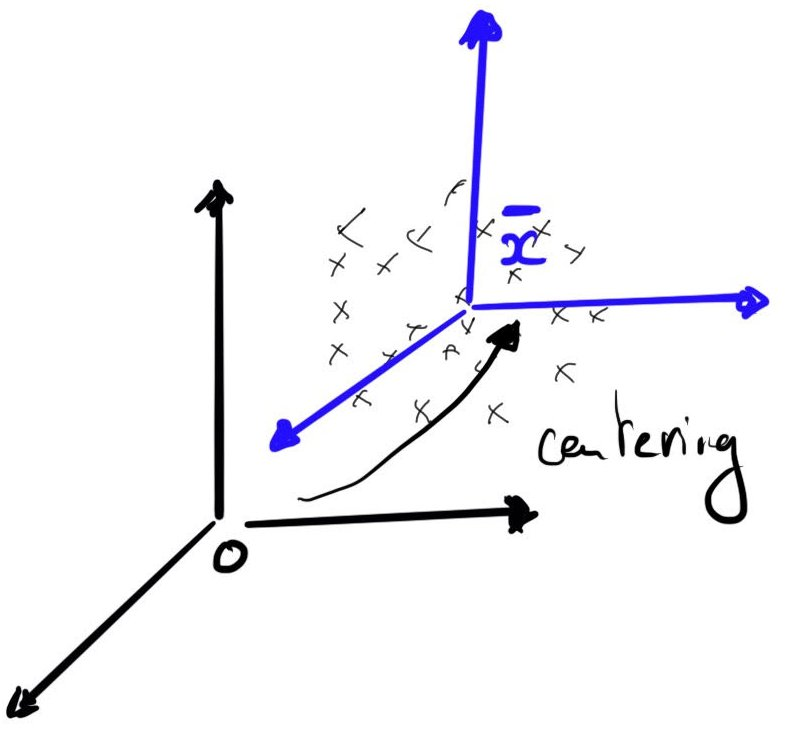
\includegraphics[width=.6\textwidth]{cloud_centering}
      \vspace{-.25cm}
      \caption{Example in $\Rset^3$}
      \end{figure}      
    \end{column}

  \begin{column}{.5\textwidth}
    \begin{block}{Center of Inertia}
      (or barycentrum, or empirical mean)
      \[ \bar{\bx} = \frac{1}{n} \sum _{i=1}^n \bx_i = 
      \begin{pmatrix}
        \sum _{i=1}^n x_{i1}/n \\
        \sum _{i=1}^n x_{i2}/n \\
        \vdots\\
        \sum _{i=1}^n x_{id} /n
      \end{pmatrix}
      \]
    \end{block}
  \end{column}
  \end{columns}

  We center the cloud $\bX$ around $\bx$ denote this by $\bX^c$
  \begin{equation*}
    \bX^c = \begin{pmatrix}
    x_{11} - \bar{x}_1 &   \dots & x_{1j}  - \bar{x}_j & \dots  & x_{1d} - \bar{x}_d   \cr
              \vdots   &  \vdots & \vdots              & \vdots & \vdots  \cr
    x_{i1} - \bar{x}_1 &   \dots & x_{ij} - \bar{x}_j  & \dots  & x_{id}  - \bar{x}_d \cr
              \vdots   &  \vdots & \vdots              & \vdots & \vdots  \cr
    x_{n1} - \bar{x}_1 &  \dots  & x_{nj} - \bar{x}_j  & \dots  & x_{nd}  - \bar{x}_d \cr
    \end{pmatrix}
  \end{equation*}

\end{frame}

\begin{frame}
  \frametitle{Inertia and Variance}

\begin{block}{Total Inertia: \textcolor{black}{distance of the individuals to the center of the cloud}}
  \[
      I_T = \frac{1}{n}\sum_{i=1}^n \sum_{j=1}^d  (x_{ij}- \bar{x}_{j}) ^2 
      = \frac{1}{n}\sum_{i=1}^n \|\bx_i - \bar{\bx} \|^2  
      = \frac{1}{n}\sum_{i=1}^n \distance^2 (\bx_i,\bar{\bx})
    \]
\end{block}

  \begin{block}{$I_T$ is proportional to the total variance}
  Let $\hat{\bSigma}$ be the empirical variance-covariance matrix
\[
      I_T = \frac{1}{n}\sum_{j=1}^p  \sum_{i=1}^n (x_{ij}- \bar{x}_{j}) ^2 
      = \sum_{j=1}^n \frac{1}{n}\|\bx^j - \bar{x}_{j} \|^2
      = \sum_{j=1}^n \var(\bx^j) = \trace{\hat{\bSigma}}
\]
\end{block}

\begin{itemize}
  \item[$\rightsquigarrow$] \alert{Good representation has large inertia} (much variability)
  \item[$\rightsquigarrow$] \alert{Large dispertion $\sim$ Large distances between points}
\end{itemize}
  
\end{frame}

\begin{frame}
  \frametitle{Inertia with respect to an axix}

  The Inertia of the cloud wrt axe $\Delta$ is the sum of the distances between all points and their orthogonal projection on $\Delta$.
  \begin{equation*}
    \begin{aligned}
      I_\Delta = \frac{1}{n}\sum_{i=1}^n \distance^2(\bx_i, \Delta)
      \end{aligned}
  \end{equation*}

  \begin{figure}
    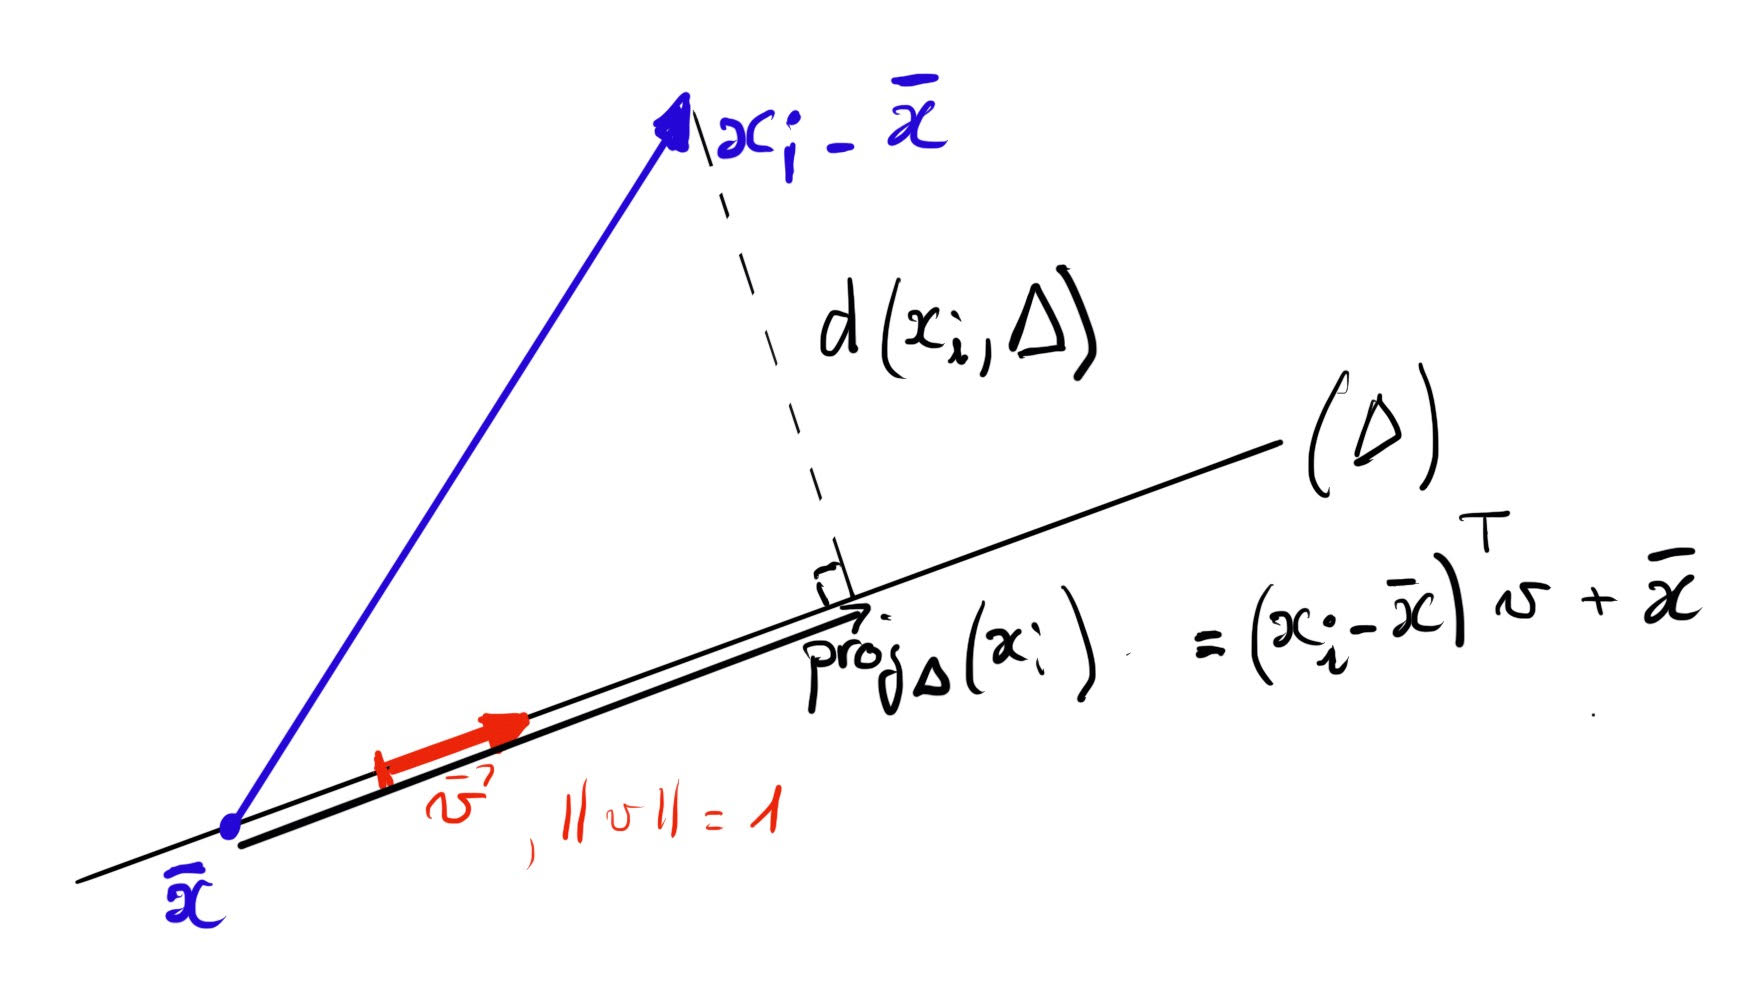
\includegraphics[width=.7\textwidth]{proj_axis}
    \caption{Projection of $\bx_i$ onto a line $\Delta$ passing through $\bar\bx$}
  \end{figure}

\end{frame}

\begin{frame}
  \frametitle{Decomposition of total Inertia (1)}
  
  Let $\Delta^\bot$ the orthogonal subspace $\Delta$  is $\Rset^n$

  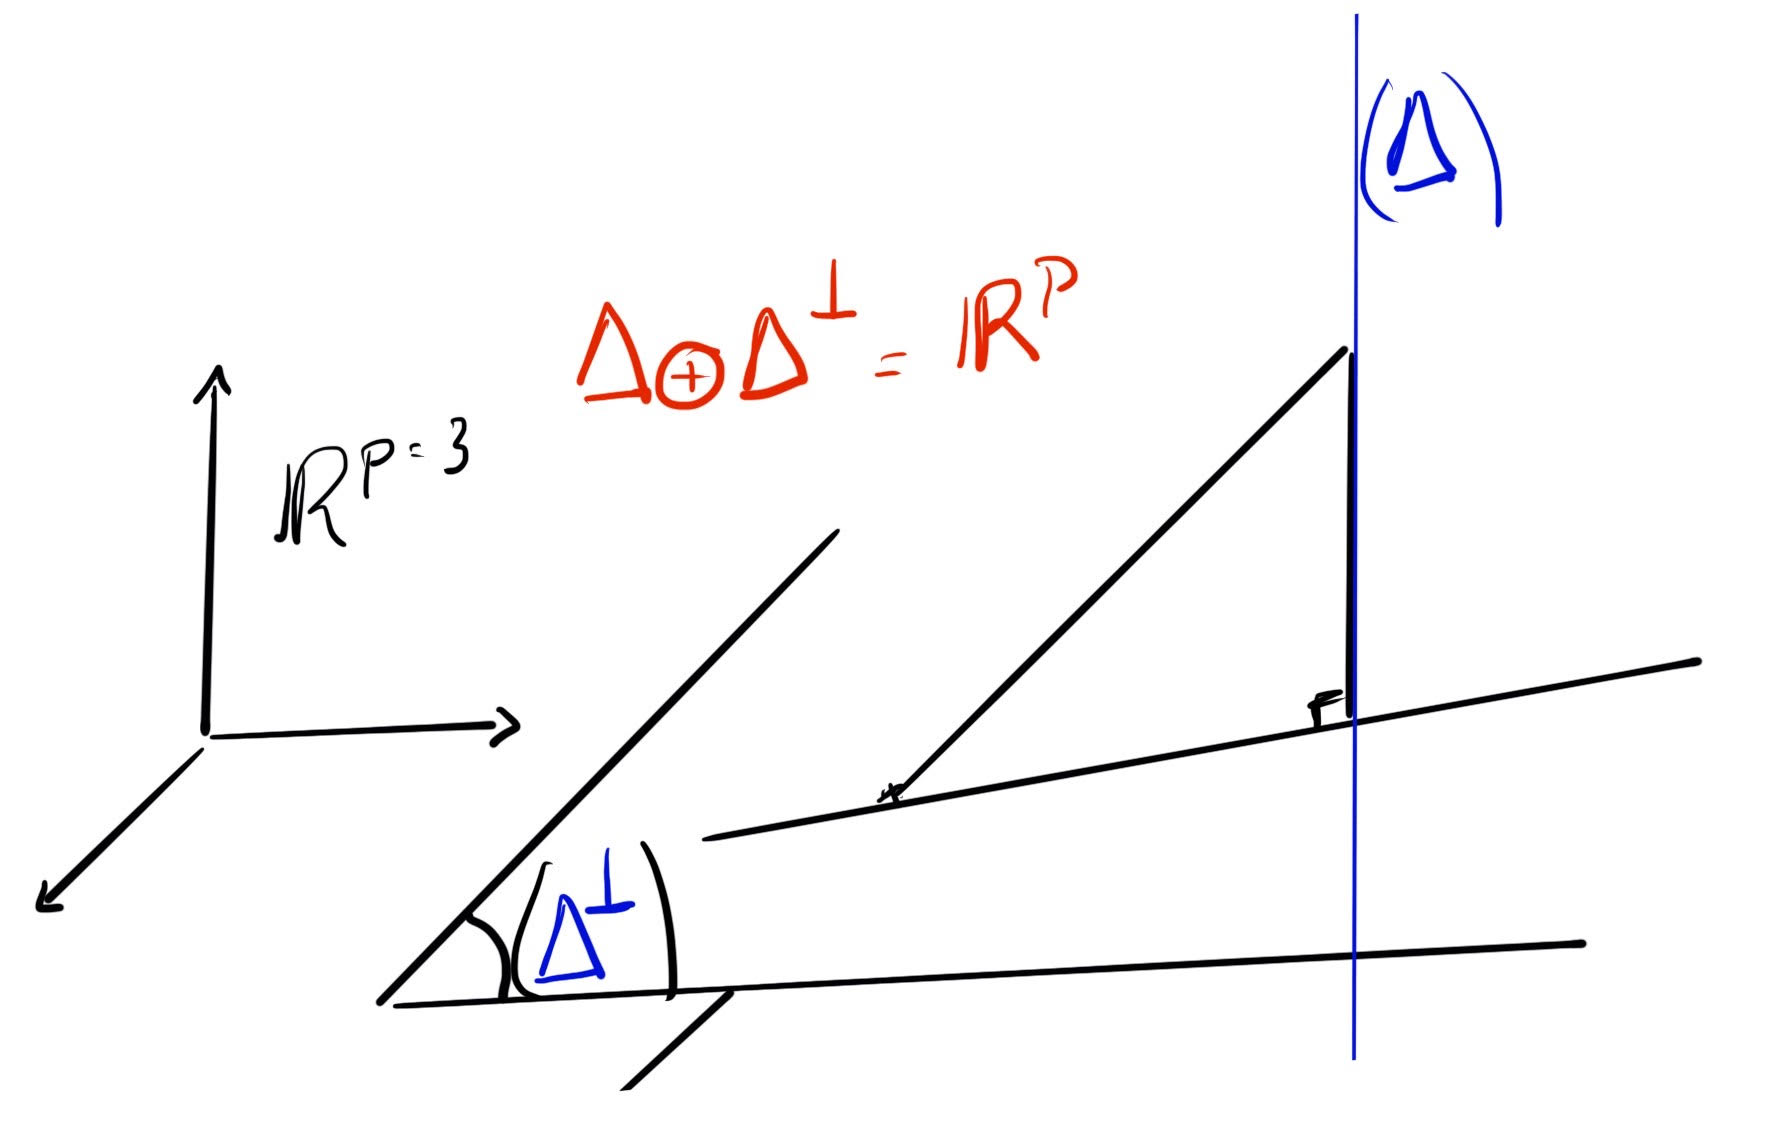
\includegraphics[width=.5\textwidth]{supp_spaces}

  \begin{block}{Theorem (Huygens)}
    A consequence of the above (Pythagoras Theorem) is the decomposition of the following total inertia:
      \begin{equation*}
        I_T = I_{\Delta} + I_{\Delta^\bot}
      \end{equation*}
    \alert{By projecting the cloud $\bX$ onto $\Delta$, with loss the inertia measured by $\Delta^\bot$}
    \end{block}
        
\end{frame}

\begin{frame}
  \frametitle{Decomposition of total Inertia (2)}
  
  Consider only subspaces with dimension $1$ (that is, lines or axes). We can decompose $\Rset^p$ the sum of $p$ othogonal axis. 
  
  \begin{equation*}
    \Rset^p = \Delta_1 \oplus \Delta_2 \oplus \dots \oplus \Delta_p
  \end{equation*}
  \alert{$\rightsquigarrow$ These axes form a new basis for representing the point cloud.}

  \begin{block}{Theorem (Huygens)}
    \begin{equation*}
      I_{T} = I_{\Delta_1} + I_{\Delta_2} + \dots + I_{\Delta_p}
    \end{equation*}
  \end{block}
  
\end{frame}
